%----------------------------------------------------------------------------------------
%	PACKAGES AND OTHER DOCUMENT CONFIGURATIONS
%----------------------------------------------------------------------------------------

% Font sizes: 10, 11, or 12;
% Paper sizes: a4paper, letterpaper, a5paper, legalpaper, executivepaper or landscape
% Font families: sans or roman
\documentclass[11pt,a4paper,sans]{moderncv}

% CV theme - options include: 'casual' (default), 'classic', 'oldstyle' and 'banking'
\moderncvstyle{banking}

% CV color - options include: 'blue' (default), 'orange', 'green', 'red', 'purple', 'grey' and 'black'
\moderncvcolor{blue}

% Reduce document margins
%\usepackage[scale=0.8]{geometry}
\usepackage[top=0.7in,bottom=0.4in,left=0.75in,right=0.75in]{geometry}
%\usepackage{minipage}

%----------------------------------------------------------------------------------------
%	Informació personal
%----------------------------------------------------------------------------------------

\firstname{Ankica}
\familyname{Peshevska}
\nationality{Nacionalidad: Macedonia -- Espa\~nola (en tr\'amite)}
\birthdate{07/02/1973}
\nie{NIE: X7501158-F}
\address{Av. Alcalde Rovira Roure 34, 1 - 4}{Lleida, Catalunya, Espa\~na 25006}
\mobile{666 39 30 16}
\phone{973 98 54 94}
\email{apesevska@yahoo.com}

\begin{document}

%----------------------------------------------------------------------------------------
%	Títol i informació personal
%----------------------------------------------------------------------------------------

\begin{minipage}[t]{0.8\textwidth}
\makecvtitle % Print the CV title
\end{minipage}
%\hspace{0.75cm}
\begin{minipage}[c]{0.175\textwidth}
%\insertphoto % Print the CV title
%\includegraphics[width=\textwidth]{pictures/picture}
{\color{color1}\framebox{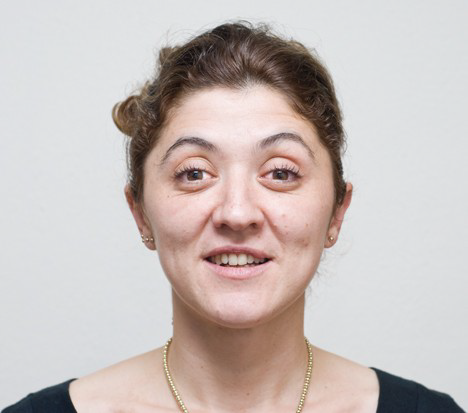
\includegraphics[width=\textwidth]{mama.png}}}
\end{minipage}
\vspace{0.75cm}

%----------------------------------------------------------------------------------------
%	Informació acadèmica
%----------------------------------------------------------------------------------------

\section{Formaci\'on acad\'emica}

\cventry{1989 -- 1991}{Bachillerato}{ETUC Koce Metalec}{Skopje}{Especialidad en electrotecnia y telecomunicaciones}{}

%----------------------------------------------------------------------------------------
%	Experiència laboral
%----------------------------------------------------------------------------------------

\section{Experiencia laboral}

%------------------------------------------------

\cventry{2015 -- febrero 2017}{Cocinera}{Restaurante Teresa Carles}{Lleida}{}{}
\cventry{2010 -- 2015}{Cocinera}{Restaurante Parad\'is}{Lleida}{}{}
\cventry{2005 -- 2009}{Camarera}{Restaurante D-Vinis}{Lleida}{}{}
\cventry{2001 -- 2004}{Administrativa}{Oficina de Correos}{Kriva Palanka, Macedonia}{}{}
\cventry{2000 -- 2001}{Cajera}{Supermercado}{Kriva Palanka, Macedonia}{}{}
\cventry{1994 -- 1995}{Camarera/relaciones p\'ublicas}{Hamburgueser\'ia Pink}{Kriva Palanka, Macedonia}{}{}
\cventry{1993}{Camarera}{Cafeter\'ia Doli}{Kriva Palanka, Macedonia}{}{}

%------------------------------------------------

%\cventry{2014}{Col$\cdot{}\!$laboraci\'o en un projecte de recerca}{\textsc{Grup de Rob\`otica, UdL}}{Lleida}{}{Col$\cdot{}\!$laboraci\'o amb el Laboratori de Rob\`otica de l'Escola Polit\`ecnica Superior en un projecte de recerca durant els mesos de Setembre i Octubre de 2014.}

%------------------------------------------------

%\cventry{Intermitent, 2009 -- 2015}{Cambrer}{\textsc{Bars i restaurants varis}}{Lleida}{}{Feines temporals durant els estius, especialment en caps de setmana.}

%----------------------------------------------------------------------------------------
%	Habilitats informàtiques
%----------------------------------------------------------------------------------------

\section{Habilidades inform\'aticas}

\cvitem{Ofim\'atica}{Redacci\'on de documentos varios (Word, Excel, PowerPoint)}
\cvitem{Corel Draw}{Dibujo y dise\~no}

%----------------------------------------------------------------------------------------
%	Idiomes
%----------------------------------------------------------------------------------------

\section{Idiomas}

\cvitemwithcomment{Macedonio}{Idioma nativo}{}
\cvitemwithcomment{Castellano}{Nivel alto}{Hablado y escrito}
\cvitemwithcomment{Catal\'an}{Nivel intermedio}{Hablado}

%----------------------------------------------------------------------------------------
%	Interessos
%----------------------------------------------------------------------------------------

\section{Otros datos de inter\'es}

\renewcommand{\listitemsymbol}{--~} % Changes the symbol used for lists
\cvitem{}{Dispongo de carn\'e de conducir B, con veh\'iculo propio}

\end{document}
